\documentclass[tikz,border=8pt]{standalone}
\usetikzlibrary{arrows.meta,positioning}
\begin{document}
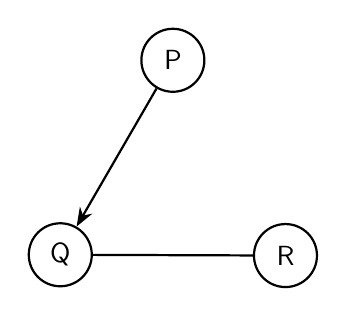
\begin{tikzpicture}[x=1cm,y=1cm]
\tikzset{
  graphnode/.style={circle,draw,thick,minimum size=8mm,inner sep=1pt,font=\sffamily},
  directed/.style={-{Stealth[length=2.4mm]},thick},
  undirected/.style={thick}
}
\node[graphnode] (n_P) at (0.00,1.65) {P};
\node[graphnode] (n_Q) at (-1.43,-0.82) {Q};
\node[graphnode] (n_R) at (1.43,-0.83) {R};
\draw[directed] (n_P) -- (n_Q);
\draw[undirected] (n_Q) -- (n_R);
\end{tikzpicture}
\end{document}
